%%%%%%%%%%%%%%%%%%%%%%%%%%%%%%%%%%%%%%%%%%%%%%%%%%%%%%%%%%%%%%%%%%%%%%%%%%%%%%%%
%2345678901234567890123456789012345678901234567890123456789012345678901234567890
%        1         2         3         4         5         6         7         8
\documentclass[letterpaper, 10 pt, conference]{ieeeconf}  % Comment this line out
% if you need a4paper
%\documentclass[a4paper, 10pt, conference]{ieeeconf}      % Use this line for a4

\usepackage{float}
% paper
% uso paquete bookmark para tener bien los outlines.
\usepackage{bookmark}

% Configuro el idioma.
\usepackage[utf8]{inputenc} % Importante para mantener acentos.
\usepackage[spanish, activeacute]{babel} % Requiere: texlive-lang-spanish. Por primera vez hay que ejecutar: texconfig init> log

% Paquete para poder usar acentos en $$.
\usepackage{mathtools}
%\setmathfont{XITS math}

\usepackage{tikz}
\usetikzlibrary{shapes.misc, positioning, shapes.geometric, arrows.meta}

\usepackage{siunitx}

% package to get \url
\usepackage{hyperref}
\hypersetup{
  colorlinks=true,
  linkcolor=magenta,
  filecolor=magenta,
  citecolor=magenta,      
  urlcolor=magenta,
}

% Graficos electrónicos
\usepackage{circuitikz}

\IEEEoverridecommandlockouts                              % This command is only
% needed if you want to
% use the \thanks command
\overrideIEEEmargins
% See the \addtolength command later in the file to balance the column lengths
% on the last page of the document

\usepackage{graphicx}
\usepackage{graphics}

% styling for matlab/octave code.
\usepackage{matlab-prettifier}
% Configuracion, con esto puede agregar ñ.
\lstset{
  literate={ñ}{{\~n}}1
}

% The following packages can be found on http:\\www.ctan.org
%\usepackage{graphics} % for pdf, bitmapped graphics files
%\usepackage{epsfig} % for postscript graphics files
%\usepackage{mathptmx} % assumes new font selection scheme installed
%\usepackage{times} % assumes new font selection scheme installed
\usepackage{amsmath} % assumes amsmath package installed
%\usepackage{amssymb}  % assumes amsmath package installed

\title{\LARGE \bf Laboratorio N° 3}

\author{
  Tom\'as Vidal\\
  {\it Circuitos Electrónicos 1}\\
  {\it Facultad de Ingenier\'ia, UNLP, La Plata, Argentina.}\\
  {\it 21 de Junio, 2024.}
}                                            % <-this % stops a space


% comienzo

% INTRO

% Figura
\newcommand{\image}[2] {
  \begin{figure}[H]
    \centering
    \includegraphics[width=0.43\textwidth]{./#1.png}
    \caption{#2}
    \label{fig:#1}
  \end{figure}
}

% Codigo
% \begin{lstlisting}[style=Matlab-editor]
% % el código va aca
% dispc("HELLO WORLD");
% \end{lstlisting}

\begin{document}
\maketitle
\thispagestyle{empty}
\pagestyle{empty}

% \section{INTRODUCCCI\'ON}
% TODO

\section{Topología presentada}
\begin{figure}[H]
 \centering
 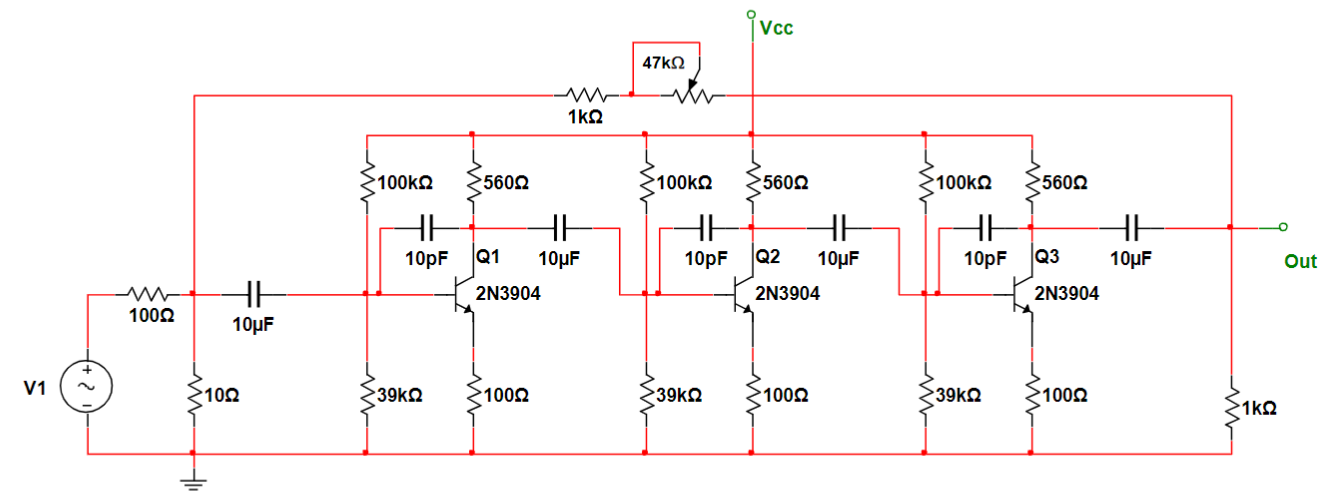
\includegraphics[width=0.43\textwidth]{./Imagenes/circuito_completo.png}
 \caption{Circuito dado}
 \label{pic:circuito_completo}
\end{figure}
\subsection{Circuito completo}
A partir del circuito dado (\ref{pic:circuito_completo}) se pueden identificar 3 etapas individuales de amplificación y una realimentación de las mismas. Por lo que a continuación se analizan estas etapas individuales y el lazo de realimentación
\subsection{Etapa aislada}
\begin{figure}[H]
  \centering
  \begin{circuitikz}
    \node[npn] (npn) at (0,0) {};
    \draw (npn.base) -- ++(-1, 0) -- ++(0, -1) to[R=$\textbf{39k}\Omega$] ++(0, -1.5) -- ++(0, -0.5) node[ground]{};
    \draw (npn.base) -- ++(-1, 0) -- ++(0, 1.5) to[R=$\textbf{100k}\Omega$] ++(0, 1.5) -- ++(0, 0.5) node[ocirc]{} coordinate (Vp) node[right, font=\large] {$+V$}; 
    \draw (npn.collector) -- ++(0, 0.75) to[R=$\textbf{560}\Omega$] ++(0, 1.5) -- ++(0, 0.5) node[ocirc]{} coordinate (Vp) node[right, font=\large] {$+V$};
    % TODO: buscar el simbolo de pico para los faradios
    \draw (npn.collector) -- ++(0, 0.5) node[circ]{} -- ++(-0.75, 0) to[C=$\textbf{10}p F$] ++(-0.5, 0) -- ++(-0.6, 0) node[circ]{};
    \draw (npn.collector) node[circ]{} -- ++(1, 0) to[C=$\textbf{10}\mu F$] ++(1, 0) -- ++(0.75, 0) node[ocirc]{} coordinate (Vin) node[right, font=\large] {$V_{s}$};
    \draw (npn.emitter) -- ++(0, -0.25) to[R=$\textbf{100}\Omega$] ++(0, -1.5) -- ++(0, -0.5) node[ground]{};
    \draw (npn.base) -- ++(-1, 0) node[circ]{} -- ++(-1, 0) to[C=$\textbf{10}\mu F$] ++(-1, 0) -- ++(-0.75, 0) node[ocirc]{} coordinate (Vin) node[left, font=\large] {$V_{e}$};
  \end{circuitikz}
  \caption{Etapa individual en el lazo directo}
  \label{circ:etapa_individual}
\end{figure}
%TODO: agregar valores de parámetros
%TODO: buscar el simbolo de pico para los faradios
Este amplificador es uno de \textit{transimpedancia} ([A/V]), y sus parámetros más representativos son: $Z_{in} = $, $Z_{out} = $, $A_{v} = $; los mismos se obtuvieron aplicando el modelo de pequeña señal del BJT, y considerando que el capacitor de $10pF$ están en circuito abierto y, los de $10\mu F$ están en cortocircuito en pequeña señal.
  

\end{document}
